  \subsection{Medición de potencia activa y factor de potencia} 
    Los conexiones explicadas se representan en el esquema de la Figura~\ref{fig:EsquemaConexiones}.
    Se hace uso de las atenuaciones que ofrece el osciloscopio digital, de forma tal que los valores
    que se miden sean exactamente los valores reales. Es decir, para el \textbf{canal 1}, en cual se mide
    la \textit{tensión de entrada} $\mathbf{V_i}$, se coloca una \textbf{atenuación x100} (x10 de la punta
    y x10 del divisor resistivo), y para el \textbf{canal 2}, en el cual se mide la \textit{corriente de entrada}
    $\mathbf{I_i}$ de forma indirecta por Ley de Ohm, se coloca una atenuación \textbf{atenuación x1}
    (debido a que $R\textsubscript{1}=10\ \Omega$).

    \begin{figure}[h]
      \centering
      \frame{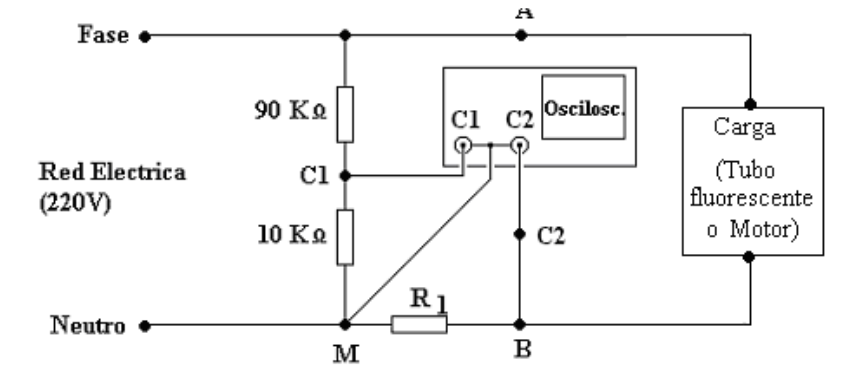
\includegraphics[width=0.8\textwidth]{Imagenes/ActividadPractica/EsquemaConexiones.png}}
      \caption{Esquema de conexiones para las mediciones.}
      \label{fig:EsquemaConexiones}
    \end{figure}
  
